% Caraumã book template by @jndgomes
% 2024 (c) Janderson Gomes
% See more <artientista.blogspot.com> or <carauman.blogspot.com>

% paper size is in preamble.sty
\documentclass[12pt,openany]{book} 

% Definindo proporção áurea
\newcommand{\goldenratio}{1.618}

% Codificação de entrada e saída
\usepackage[T1]{fontenc}
\usepackage{hyperref}

% Informações do livro
\newcommand{\authorname}{S1e7J}
\newcommand{\translatorname}{Sergio Montoya Ramirez}
\newcommand{\booktitle}{Titulo del Libro}
\newcommand{\subtitle}{Subtitulo}
\newcommand{\publisher}{Caraumã}
\newcommand{\editionyear}{2025}
\newcommand{\isbn}{}
\title{\booktitle}
\author{\authorname}

% Pacotes adicionais
\usepackage{misc/options}

\begin{document}

% Front matter
\frontmatter
\pagestyle{empty}

% Capa
\begin{center}
\begin{tikzpicture}[remember picture,overlay]

    % Proporção áurea
    %\pgfmathsetmacro{\goldenheight}{\paperwidth / \goldenratio}
    %\pgfmathsetmacro{\goldenwidth}{\paperwidth}

    % Fundo preto
    \fill[black] (current page.south west) rectangle (current page.north east);

    % Autor
    \node[white, font=\Huge, anchor=north, text width =\linewidth, align = center] (author) at ([yshift=-44pt] current page.north) {\textcolor{customgold}{\scshape\large\authorname}};

    % Título
    \node[white, font=\Large, anchor=north, text width =0.9\linewidth, align = center, below=4pt of author.south] (title) {\scshape\Huge\booktitle};

    % Subtítulo
    \ifx\subtitle\undefined\else\if\relax\detokenize\expandafter{\subtitle}\relax\else
    {\node[white, font=\Large, text width =\linewidth, align = center, anchor=north, below=8pt of title.south] {\textcolor{lightgray}{\scshape\large\subtitle}};}
    \fi\fi

    % Padrão de círculos central
    \begin{scope}[shift={(current page.center)}, scale=1.0871]
        \foreach \x in {-20, -18, -16, -14, -12, -10, -8, -6, -4, -2, 0, 2, 4, 6, 8, 10, 12, 14, 16, 18} {
            \foreach \y in {-2, 2} {
                \begin{scope}[shift={(\x + 1, \y)}]
                    \foreach \r in {0.2, 0.4, 0.6, 0.8, 1.0} {
                        \draw[thick, darkgray] (0,0) circle (\r);
                    }
                \end{scope}
            }
            \foreach \y in {-3, -1, 1, 3} {
                \begin{scope}[shift={(\x, \y)}]
                    \foreach \r in {0.2, 0.4} {
                        \draw[thick, darkgray] (0,0) circle (\r);
                    }
                \end{scope}
            }
            \foreach \y in {-1, 1} {
                \begin{scope}[shift={(\x, 0)}]
                    \foreach \r in {0.2, 0.4, 0.6, 0.8, 1.0} {
                        \draw[thick, customgold] (0,0) circle (\r);
                        \fill[thick, customgold] (0,0) circle (\r);
                    }
                \end{scope}
            }
            \foreach \y in {-1, 1} {
                \begin{scope}[shift={(\x, \y)}]
                    \foreach \r in {0.2, 0.4, 0.6, 0.8, 1.0} {
                        \fill[black] (0,0) circle (\r);
                    }
                \end{scope}
            }
            \foreach \y in {-1, 1} {
                \begin{scope}[shift={(\x, \y)}]
                    \foreach \r in {0.2, 0.4, 0.6, 0.8, 1.0} {
                        \draw[thick, darkgray] (0,0) circle (\r);
                    }
                \end{scope}
            }
        }
    \end{scope}

    % Editora
    \node[white, font=\Huge, anchor=south] (publisher) at ([yshift=32pt] current page.south) {\textcolor{gray}{\scshape\large\publisher}};

    % Logotipo da editora
    \node[anchor=north, above=4pt of publisher.north] {
\includegraphics[width=0.07\textwidth]{frontmatter/logo-white.png}};

    % Outras informações
    \ifx\translatorname\undefined
    \else
        \if\relax\detokenize\expandafter{\translatorname}\relax
        \else{   
            \node[white, font=\Large, anchor=north, above=114pt of publisher.north] (translatedBy) {\textcolor{gray}{\itshape\large{Traducción por}}};
            
            \node[white, font=\Large, anchor=south, below=2pt of translatedBy.south] (translatorAuthor) {\textcolor{lightgray}{\itshape\large\translatorname}};       
            }
        \fi
    \fi        
\end{tikzpicture}
\end{center}

\cleardoublepage

% Página de título (contra-capa)
\begin{titlepage}
	\centering
	\newgeometry{top=1in,bottom=1in,right=0in,left=0in}
    \thispagestyle{empty}
	~	
    % Autor
	\vspace{24pt}
	{\scshape\large \authorname\par}

    % Título
	\vspace{6pt}
	{\scshape\Huge \booktitle\par}

    % Subtítulo
    \ifx\subtitle\undefined\else\if\relax\detokenize\expandafter{\subtitle}\relax\else
    {\vspace{6pt}
	{\scshape\large \subtitle\par}
 
	\vspace{\stretch{1.25}}}
    \fi\fi
    
    % Quem fez a tradução
    \ifx\translatorname\undefined\else\if\relax\detokenize\expandafter{\translatorname}\relax\else
    {{\itshape\large{Traducción por}\par}
	\vspace{6pt}

    {\itshape\Large\translatorname\par}}
    \fi\fi

    % Editora
    \vspace{\stretch{6}}
	{\Huge\scshape\large\publisher\par}
\end{titlepage}
      % Página de título
% Página de copyright

{\small
\setlength{\parindent}{0em}\setlength{\parskip}{1em}
~
\vfill

% Data da primeira publicação
Primera edición, \editionyear{}

% Copyright
Copyright \copyright{} 2025 \authorname

% Texto resumido da licença

Todo el contenido de esta publicación está licenciado bajo la Licencia Creative Commons Atribución-NoComercial-SinDerivadas 4.0 Internacional. Usted está autorizado a compartir, copiar y redistribuir el material en cualquier formato o medio, siempre que atribuya crédito al autor original, no modifique el contenido de ninguna forma, no utilice este trabajo para fines comerciales. Para más detalles sobre los términos de esta licencia, visite http://creativecommons.org/licenses/by-nc-nd/4.0/.  

% ISBN, se houver
\ifx\isbn\undefined\else\if\relax\detokenize\expandafter{\isbn}\relax\else{ISBN \isbn{}}\fi\fi

% Logotipo da editora
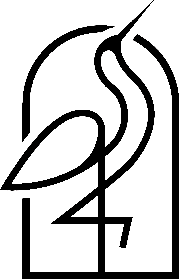
\includegraphics[width=0.07\linewidth]{frontmatter/logo-black.png}

% Editora
Publicado por \publisher{}
}
  % Página de direitos autorais
% Prefácio
\chapter{Prefácio}

\lettrine{L}{orem ipsum dolor sit amet}, consectetuer adipiscing elit. Etiam lobortis facilisis sem. Nullam nec mi et neque pharetra sollicitudin. Praesentimperdiet mi nec ante. Donec ullamcorper, felis non sodales commodo, lectus velit ultrices augue, a dignissim nibh lectus placerat pede. Vivamus nunc nunc, molestie ut, ultricies vel, semper in, velit. Ut porttitor. Praesent in sapien. Lorem ipsum dolor sit amet, consectetuer adipiscing elit. Duis fringilla tristique neque. Sed interdum libero ut metus. Pellentesque placerat. Nam rutrum augue a leo. Morbi sed elit sit amet antelobortis sollicitudin. Praesent blandit blandit mauris. Praesent lectustellus, aliquet aliquam, luctus a, egestas a, turpis. Mauris lacinia loremsit amet ipsum. Nunc quis urna dictum turpis accumsan semper.

Lorem ipsum dolor sit amet, consectetuer adipiscing elit. Etiam lobortis facilisis sem. Nullam nec mi et neque pharetra sollicitudin. Praesentimperdiet mi nec ante. Donec ullamcorper, felis non sodales commodo, lectus velit ultrices augue, a dignissim nibh lectus placerat pede. Vivamus nunc nunc, molestie ut, ultricies vel, semper in, velit. Ut porttitor. Praesent in sapien. Lorem ipsum dolor sit amet, consectetuer adipiscing elit. Duis fringilla tristique neque. Sed interdum libero ut metus. Pellentesque placerat. Nam rutrum augue a leo. Morbi sed elit sit amet antelobortis sollicitudin. Praesent blandit blandit mauris. Praesent lectustellus, aliquet aliquam, luctus a, egestas a, turpis. Mauris lacinia loremsit amet ipsum. Nunc quis urna dictum turpis accumsan semper.

Lorem ipsum dolor sit amet, consectetuer adipiscing elit. Etiam lobortis facilisis sem. Nullam nec mi et neque pharetra sollicitudin. Praesentimperdiet mi nec ante. Donec ullamcorper, felis non sodales commodo, lectus velit ultrices augue, a dignissim nibh lectus placerat pede. Vivamus nunc nunc, molestie ut, ultricies vel, semper in, velit. Ut porttitor. Praesent in sapien. Lorem ipsum dolor sit amet, consectetuer adipiscing elit. Duis fringilla tristique neque. Sed interdum libero ut metus. Pellentesque placerat. Nam rutrum augue a leo. Morbi sed elit sit amet antelobortis sollicitudin. Praesent blandit blandit mauris. Praesent lectustellus, aliquet aliquam, luctus a, egestas a, turpis. Mauris lacinia loremsit amet ipsum. Nunc quis urna dictum turpis accumsan semper.

Lorem ipsum dolor sit amet, consectetuer adipiscing elit. Etiam lobortis facilisis sem. Nullam nec mi et neque pharetra sollicitudin. Praesentimperdiet mi nec ante. Donec ullamcorper, felis non sodales commodo, lectus velit ultrices augue, a dignissim nibh lectus placerat pede. Vivamus nunc nunc, molestie ut, ultricies vel, semper in, velit. Ut porttitor. Praesent in sapien. Lorem ipsum dolor sit amet, consectetuer adipiscing elit. Duis fringilla tristique neque. Sed interdum libero ut metus. Pellentesque placerat. Nam rutrum augue a leo. Morbi sed elit sit amet antelobortis sollicitudin. Praesent blandit blandit mauris. Praesent lectustellus, aliquet aliquam, luctus a, egestas a, turpis. Mauris lacinia loremsit amet ipsum. Nunc quis urna dictum turpis accumsan semper.

Lorem ipsum dolor sit amet, consectetuer adipiscing elit. Etiam lobortis facilisis sem. Nullam nec mi et neque pharetra sollicitudin. Praesentimperdiet mi nec ante. Donec ullamcorper, felis non sodales commodo, lectus velit ultrices augue, a dignissim nibh lectus placerat pede. Vivamus nunc nunc, molestie ut, ultricies vel, semper in, velit. Ut porttitor. Praesent in sapien. Lorem ipsum dolor sit amet, consectetuer adipiscing elit. Duis fringilla tristique neque. Sed interdum libero ut metus. Pellentesque placerat. Nam rutrum augue a leo. Morbi sed elit sit amet antelobortis sollicitudin. Praesent blandit blandit mauris. Praesent lectustellus, aliquet aliquam, luctus a, egestas a, turpis. Mauris lacinia loremsit amet ipsum. Nunc quis urna dictum turpis accumsan semper.

\cleardoublepage   % Make sure contents page starts on right-side page        % Prefácio
\tableofcontents\thispagestyle{empty}\cleardoublepage        % Sumário

% Main matter
\pagestyle{fancy}                  % Estilo de página fancy para o conteúdo principal

% Conteúdo dos capítulos
\mainmatter
\chapter{Bitacora}
\section{Primer Dia: Sisifo Observa la Montaña}
\emph{08 de Mayo de 2025}

Llevo programando ya casi 5 años y de ellos los proyectos mas largos que he hecho
son como maximo de 2000 lineas de codigo. Creo que se me da bien pero la verdad es que
ya estoy algo cansado de los proyectos pequeños. Por lo tanto hoy asumi un nuevo reto.

Voy a hacer un lenguaje de programación con el que hacer metodos formales. Debo ser
honesto, el titulo de esta entrada es, cuando mucho, un deseo. No soy Sisifo viendo
la montaña que se me viene. Pero intentar acotar un proyecto asi de grande antes de
siquiera iniciar suele ser una gran
excusa para procrastinar (y creanme que en eso si soy experto). Asi que no hay mas que mirar
que simplemente ponerse los guantes y salir a ver que se encuentra.

Con esta mentalidad decidi que lo primero que queria hacer era aprender a programar un
lenguaje perse. En este momento debo sincerarme. Nunca he hecho un compilador. He hecho
transpiladores (y varios de ellos) ademas de un par de interpretes (entre los que estan
mas interpretes de BrainF*ck de lo que suele ser una buena idea). Por lo tanto me siento
relativamente tranquilo con el front-end de un compilador. Ahora bien, el back-end es para
mi un misterio aun. Por lo tanto doy por iniciado con este articulo la etapa de exploración
de este proyecto. Esta etapa consistira en programar la mayor cantidad de compiladores que
pueda para considerar diferentes posibilidades. Iniciare por un tutorial para crear scheme
\footnote{\url{https://en.wikibooks.org/wiki/Write_Yourself_a_Scheme_in_48_Hours}} en
Haskell solamente para probar y seguire asi durante un mes. El objetivo es en este mes
haber hecho por lo menos 3 proyectos distintos en donde haya construido 3 lenguajes de
programación diferentes. Como se imaginaran esto tomara mucho tiempo por cada uno asi que
tengo que comprometerme. Ya el dia de hoy inicie un
poco\footnote{Se que suena sospechoso pero aun no pienso subirlo a github hasta que no avance otro poco aun cuando ya estoy usando git para hacer su seguimiento. Cuando lo sienta en mejores condiciones lo subire}
con un parser para Scheme pero aun estoy lejos de conseguir algo interesante.

Ahora bien, quiero confesar que este no va a ser el unico medio por el que lo pondre. Mi objetivo es
cada semana (el fin de semana) grabar un video en el cual cuento que hice esa semana y por que me parece
muy interesante. No creo que sea un video particularmente producido aunque quien sabe si me de la
chiripiorca despues. A fin de cuentas este es un proyecto solamente por aprender asi que no me niego
a nada de lo que el viento me traiga. Hoy es miercoles asi que aun tengo un poco de tiempo para
el primer video pero la verdad es que las ganas de que esto salga bien me mueven todo el cuerpo.

Espero seguir contandoles mas a medida que el tiempo pasa. Nos vemos despues.

\pagebreak
\section{A veces avanzar se ve pequeño}
\emph{09 de Mayo de 2025}

Hoy avance poco en el proyecto. La universidad, los trabajos y proyectos personales me mantuvieron al borde de no poder avanzar mas. Sin embargo, avance. A veces avanzar no es gastar 8 horas leyendo y programando como ayer si no que se ve como hoy. A veces avanzar se ve pequeño, minusculo incluso. 5 lineas de codigo en las que invertiste 30 minutos. Pero esos minutos son mas que las 5 lineas que escribiste. A veces avanzar es simplemente la excusa para que mañana no sea tan dificil avanzar un poco mas. Creo que el problema con el que me he enfrentado antes es que soy capaz de someterme a mucho esfuerzo por periodos cortos de tiempo. Trabajar seguido se me da bien y puedo trabajar mas de 10 horas (de trabajo real) en un dia. Pero cuando me enfrento a un proyecto tan grande como este creo que hay valor en verlo como lo que es. Un proceso lento y en donde 30 minutos al dia puede ser lo unico que tenga para ofrecer algunos dias. Aun tengo mucho por trabajar y espero poder avanzar mas el fin de semana pero me quiero dar tranquilidad y paciencia mientras lo hago. De nada sirve quemarme temprano cuando el objetivo recide tan lejos.


% Capítulo I
\chapter{Primer Capitulo}

% Conteúdo do primeiro capítulo
\lettrine{L}{orem ipsum dolor sit amet}, consectetuer adipiscing elit. Etiam lobortis facilisis sem. Nullam nec mi et neque pharetra sollicitudin. Praesentimperdiet mi nec ante. Donec ullamcorper, felis non sodales commodo, lectus velit ultrices augue, a dignissim nibh lectus placerat pede. Vivamus nunc nunc, molestie ut, ultricies vel, semper in, velit. Ut porttitor. Praesent in sapien. Lorem ipsum dolor sit amet, consectetuer adipiscing elit. Duis fringilla tristique neque. Sed interdum libero ut metus. Pellentesque placerat. Nam rutrum augue a leo. Morbi sed elit sit amet antelobortis\footnote{Lorem ipsum dolor sit amet, consectetuer adipiscing elit. Etiam lobortis facilisis sem. Nullam nec mi et neque pharetra sollicitudin.} sollicitudin. Praesent blandit blandit mauris. Praesent lectustellus, aliquet aliquam, luctus a, egestas a, turpis. Mauris lacinia loremsit amet ipsum. Nunc quis urna dictum turpis accumsan semper.

Lorem ipsum dolor sit amet, consectetuer adipiscing elit. Etiam lobortis facilisis sem. Nullam nec mi et neque pharetra sollicitudin. Praesentimperdiet mi nec ante. Donec ullamcorper, felis non sodales commodo, lectus velit ultrices augue, a dignissim nibh lectus placerat pede. Vivamus nunc nunc, molestie ut, ultricies vel, semper in, velit. Ut porttitor. Praesent in sapien. Lorem ipsum dolor sit amet, consectetuer adipiscing elit. Duis fringilla tristique neque. Sed interdum libero ut metus. Pellentesque placerat. Nam rutrum augue a leo. Morbi sed elit sit amet antelobortis sollicitudin. Praesent blandit blandit mauris. Praesent lectustellus, aliquet aliquam, luctus a, egestas a, turpis. Mauris lacinia loremsit amet ipsum. Nunc quis urna dictum turpis accumsan semper.

Lorem ipsum dolor sit amet, consectetuer adipiscing elit. Etiam lobortis facilisis sem. Nullam nec mi et neque pharetra sollicitudin. Praesentimperdiet mi nec ante. Donec ullamcorper, felis non sodales commodo, lectus velit ultrices augue, a dignissim nibh lectus placerat pede. Vivamus nunc nunc, molestie ut, ultricies vel, semper in, velit. Ut porttitor. Praesent in sapien. Lorem ipsum dolor sit amet, consectetuer adipiscing elit. Duis fringilla tristique neque. Sed interdum libero ut metus. Pellentesque placerat. Nam rutrum augue a leo. Morbi sed elit sit amet antelobortis sollicitudin. Praesent blandit blandit mauris. Praesent lectustellus, aliquet aliquam, luctus a, egestas a, turpis. Mauris lacinia loremsit amet ipsum. Nunc quis urna dictum turpis accumsan semper.

Lorem ipsum dolor sit amet, consectetuer adipiscing elit. Etiam lobortis facilisis sem. Nullam nec mi et neque pharetra sollicitudin. Praesentimperdiet mi nec ante. Donec ullamcorper, felis non sodales commodo, lectus velit ultrices augue, a dignissim nibh lectus placerat pede. Vivamus nunc nunc, molestie ut, ultricies vel, semper in, velit. Ut porttitor. Praesent in sapien. Lorem ipsum dolor sit amet, consectetuer adipiscing elit. Duis fringilla tristique neque. Sed interdum libero ut metus. Pellentesque placerat. Nam rutrum augue a leo. Morbi sed elit sit amet antelobortis sollicitudin. Praesent blandit blandit mauris. Praesent lectustellus, aliquet aliquam, luctus a, egestas a, turpis. Mauris lacinia loremsit amet ipsum. Nunc quis urna dictum turpis accumsan semper.

Lorem ipsum dolor sit amet, consectetuer adipiscing elit. Etiam lobortis facilisis sem. Nullam nec mi et neque pharetra sollicitudin. Praesentimperdiet mi nec ante. Donec ullamcorper, felis non sodales commodo, lectus velit ultrices augue, a dignissim nibh lectus placerat pede. Vivamus nunc nunc, molestie ut, ultricies vel, semper in, velit. Ut porttitor. Praesent in sapien. Lorem ipsum dolor sit amet, consectetuer adipiscing elit. Duis fringilla tristique neque. Sed interdum libero ut metus. Pellentesque placerat. Nam rutrum augue a leo. Morbi sed elit sit amet antelobortis sollicitudin. Praesent blandit blandit mauris. Praesent lectustellus, aliquet aliquam, luctus a, egestas a, turpis. Mauris lacinia loremsit amet ipsum. Nunc quis urna dictum turpis accumsan semper.
           % Capítulo 1

% Back matter
\backmatter
\pagestyle{empty}

\cleardoublepage

% Capa do verso do livro
\begin{center}
\begin{tikzpicture}[remember picture,overlay]
    
    % Fundo preto
    \fill[black] (current page.south west) rectangle (current page.north east);    

    % Padrão de círculos central
    \begin{scope}[shift={(current page.center)}, scale=1.0871]
        \foreach \x in {-20, -18, -16, -14, -12, -10, -8, -6, -4, -2, 0, 2, 4, 6, 8, 10, 12, 14, 16, 18} {
            \foreach \y in {-2, 2} {
                \begin{scope}[shift={(\x + 1, \y)}]
                    \foreach \r in {0.2, 0.4, 0.6, 0.8, 1.0} {
                        \draw[thick, darkgray] (0,0) circle (\r);
                    }
                \end{scope}
            }
            \foreach \y in {-3, -1, 1, 3} {
                \begin{scope}[shift={(\x, \y)}]
                    \foreach \r in {0.2, 0.4} {
                        \draw[thick, darkgray] (0,0) circle (\r);
                    }
                \end{scope}
            }
            \foreach \y in {-1, 1} {
                \begin{scope}[shift={(\x, 0)}]
                    \foreach \r in {0.2, 0.4, 0.6, 0.8, 1.0} {
                        \draw[thick, lightgray] (0,0) circle (\r);
                    }
                \end{scope}
            }
            \foreach \y in {-1, 1} {
                \begin{scope}[shift={(\x, \y)}]
                    \foreach \r in {0.2, 0.4, 0.6, 0.8, 1.0} {
                        \fill[black] (0,0) circle (\r);
                    }
                \end{scope}
            }
            \foreach \y in {-1, 1} {
                \begin{scope}[shift={(\x, \y)}]
                    \foreach \r in {0.2, 0.4, 0.6, 0.8, 1.0} {
                        \draw[thick, darkgray] (0,0) circle (\r);
                    }
                \end{scope}
            }
        }
    \end{scope}

    % Título
    \node[white, anchor=north, text width =0.9\linewidth, align = justify] at ([yshift=-48pt] current page.north) {\scshape{Lorem ipsum dolor sit amet, consectetuer adipiscing elit. Etiam lobortis facilisis sem. Nullam nec mi et neque pharetra sollicitudin. Praesentimperdiet mi nec ante. Donec ullamcorper, felis non sodales commodo, lectus velit ultrices augue, a dignissim nibh lectus placerat pede. Vivamus nunc nunc, molestie ut, ultricies vel, semper in, velit.}};

    % Logotipo da editora
    \node[anchor=north, above=4pt of publisher.north] {
\includegraphics[width=0.07\textwidth]{frontmatter/logo-white.png}};

\end{tikzpicture}
\end{center}
       % Página final (contracapa)

\end{document}
